\begin{figure}
  \centering
  \subfigure[Overloaded semantics: The cloud and tree have similar
             shapes but different meanings due to context.] {
    \label{fig:cloud-1} 
    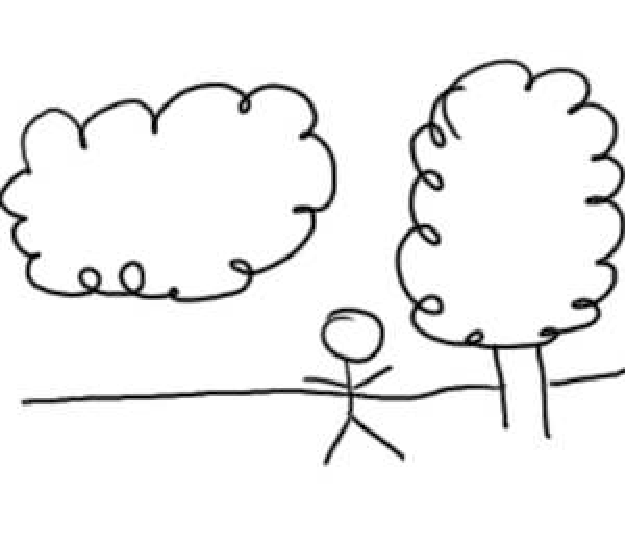
\includegraphics[width=0.25\linewidth]{img/cloud-1.pdf} 
  }
  \hspace{0.03\linewidth}
  \subfigure[Ambiguity: Changing the drawing slightly changes our
             interpretation. The object on the left may be a cloud, or
             it may be a cartoon thought bubble.] { 
    \label{fig:cloud-2} 
    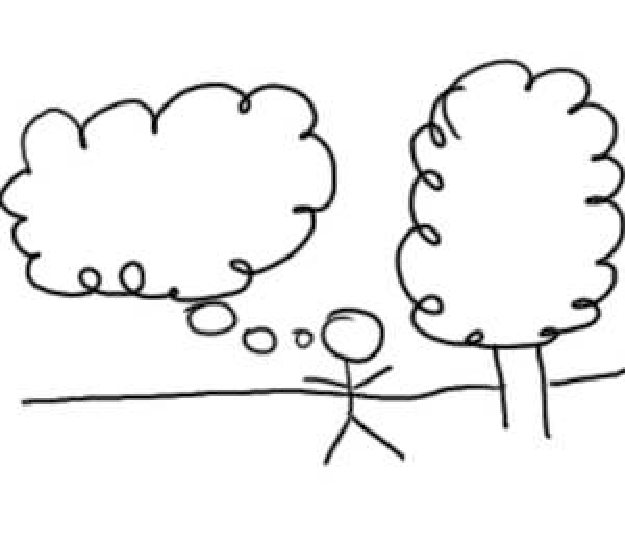
\includegraphics[width=0.25\linewidth]{img/cloud-2.pdf} 
  }
  \hspace{0.03\linewidth}
  \subfigure[Additional information helps us reason about the intended
             identity of elements. Text inside the cloud indicates it
             is a cartoon thought bubble.]  {
    \label{fig:cloud-3} 
    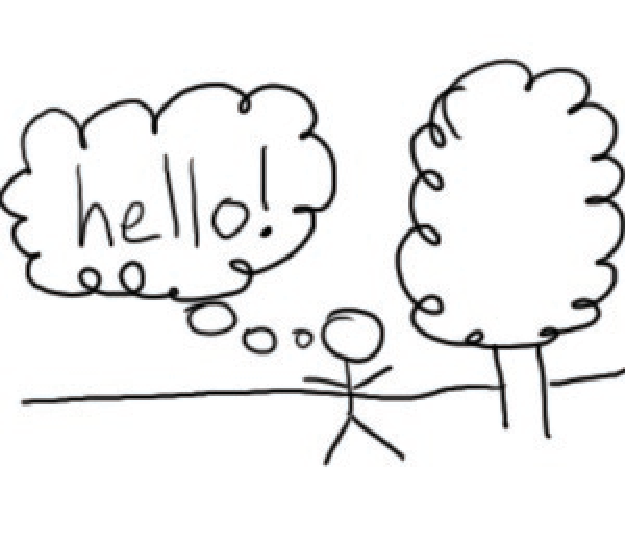
\includegraphics[width=0.25\linewidth]{img/cloud-3.pdf} 
  }
  \caption[Overloaded semantics and ambiguity]{Overloaded semantics
    and ambiguity.}
  \label{fig:cloud}
\end{figure}
